% Proposed Scheme
\section{Proposed Scheme}
The proposed scheme of this project included 5 main phases for developing a diet recommendation system using machine learning. Here’s a brief explanation of the steps.

\begin{enumerate}
    \item \textbf{Data Collection}: This step involved collecting the data from online websites.
    \item \textbf{Data Preprocessing}: This step involved organizing the dataset, extracting the input features needed, and separating the data to be used in the training, validation, and testing phases.
    \item \textbf{Model Development}: This step involved selecting a machine learning technique, Multi-layer Perceptron and neural networks in our example, setting up the network architecture (input, hidden, and output neurons), and training the network to learn the relationship between inputs and outputs with the help of our training data.
    \item \textbf{Model Testing}: This step involved validating and testing our trained neural network with the help of our testing data.
    \item \textbf{Performance Evaluation}: This step involved analyzing the performance of the trained neural network through accuracy and loss graphs by comparing predicted vs actual outputs to evaluate how accurate our model is.
\end{enumerate}

\begin{figure}
    \centering
    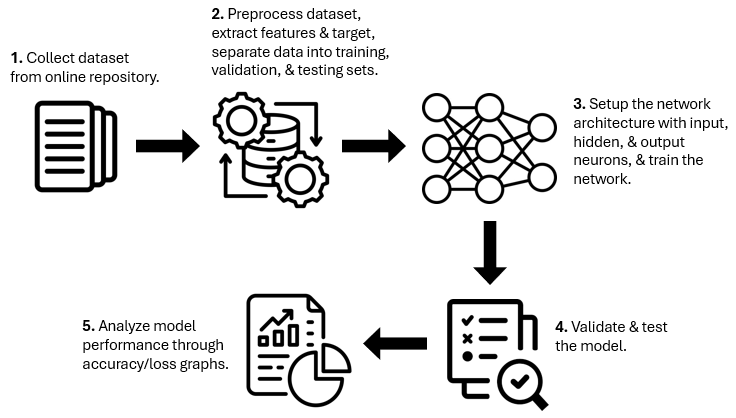
\includegraphics[width=\linewidth]{Figures/proposed scheme 2.png}
    \caption{Illustration of the proposed scheme}
\end{figure}